


\part{Entendiendo el Simulador simusched}

\section{Ejercicio 1}

Implementamos el Metodo TaskCon segun lo pedido.

\begin{framed}
\begin{verbatimtab}
void TaskCon(vector<int> params) { // params: 3
	int n = params[0];
	int bmin = params[1];
	int bmax = params[2];
	
	// INICIALIZAMOS SEMILLA DE RAND()
	srand ( time(NULL) );
	
	for( int i = 0; i < n ; i++ ) {
		int time = bmin;
		if(bmin != bmax)
			time = (rand()%(bmax-bmin+1))+bmin;
		uso_IO(time);
	}
}
\end{verbatimtab}
\end{framed}

\section{Ejercicio 2}

Creamos el archivo \verb|ejercicio2.tsk|

\begin{framed}
\begin{verbatim}
# FILE ejercicio2.tsk
TaskCPU 10
@1
TaskCon 10 1 4
@3
TaskCon 7 1 3
\end{verbatim}
\end{framed}


Luego ejecutamos Simusched con los siguientes parametros:

\begin{framed}
\begin{verbatim}
./simusched ejercicio2.tsk 1 SchedFCFS | python graphsched.py > ejercicio2.png
\end{verbatim}
\end{framed}

\begin{figure}[h!]
  \caption{Una tarea de uso intensivo del procesador y dos interactivas con Scheduling FCFS.}
  \centering
    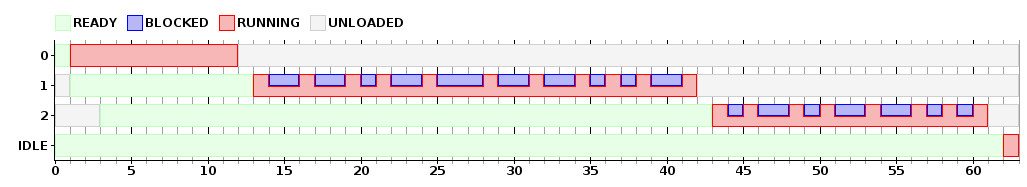
\includegraphics[width=1\textwidth]{img/ejercicio2.png}
\end{figure}


